\section{Sécurisation du drone}
Comme nous avons pu le voir, cet AR Drone 2.0 de Parrot rencontre de nombreux problèmes de sécurité et reste vulnérable a certaines attaques. L'une des vulnérabilité principale se trouve dans le point d'accès Wifi qui est un réseau ouvert donc accessible à toute personne se trouvant à portée du drone.

\subsection{Sécurisation via le Wifi}
\paragraph{Modification du point d'accès}
L'une des premières mesures pour ce drone serait donc une modification de ce point d'accès Wifi en y ajoutant un mot de passe afin de le rendre privée. Afin de minimiser les risques de compromission du réseau, l'utilisation de la norme WPA2 semble optimale. Après un rapide état de l'art sur internet, il semblerait que personne ne se soit réellement pencher sur le problème mais un fichier bash présent sur le réseau, \textit{nom du fichier}, laisse présager que cette modification est possible.

\paragraph{Utilisation du drone comme un client}
Une autre solution consisterait à utiliser le drone non comme un point d'accès mais comme un client du Wifi.
Afin de pouvoir connecter le drone à un réseau en WPA2, il est nécessaire d'effectuer de la compilation croisée sur le module \textit{wpa\_supplicant}, qui gère les connections au wifi WPA2 sur les environement Unix. En effet, le drone possède un architecture ARM et non x86. Heureusement, la communauté est riche de talent, et ce travail à déjà était fait dans ce dépot Github: \url{https://github.com/daraosn/ardrone-wpa2}.

Cette manipulation se fait en plusieurs étapes:
\begin{itemize}
  \item installation du module \textit{wpa\_supplicant} sur le drone.
  \item conecter le drone au point d'accès WPA2 du téléphone.
  \item faire en sorte que le drone est l'adresse 192.168.1.1. Changer l'adresse du point d'accès pour le permettre.
  \item contrôler le drone via le téléphone.
\end{itemize}

Avec ce procédé, on bénéficie alors d'une connexion sécurisée avec le drone que l'on pilote. Attention toutefois à bien choisir son mot de passe. En effet, si une personne arrive à se connecter au Wifi du téléphone, le drone redevient totalement vulnérable. La contrainte de cette techique est donc l'utilisation d'un point d'accès wifi annexe avec la bonne adresse ip pour le routeur. Dans un premier temps, nous l'avons essayer rapidement avec un iPhone comme point d'accès mais celui-ci n'offre pas un réseau interne du type \textit{191.168.1.0/24} et il n'est pas possible de modifier cela dans les paramètres.

\section{Connection à distance}
Comme vu précédemment, le drone dispose de 3 services tcp ouvert dont le service \textbf{ftp} et le service \textbf{telnet}. Ces deux service sont très utiles pour la dépose de fichier où encore la maintenance du drone à distance. Mais ils représentes surtout 2 portes ouvertes sur le drone et sont donc de réelles menaces pour la sécurité du drone.

\begin{figure}[H]
  \centering
  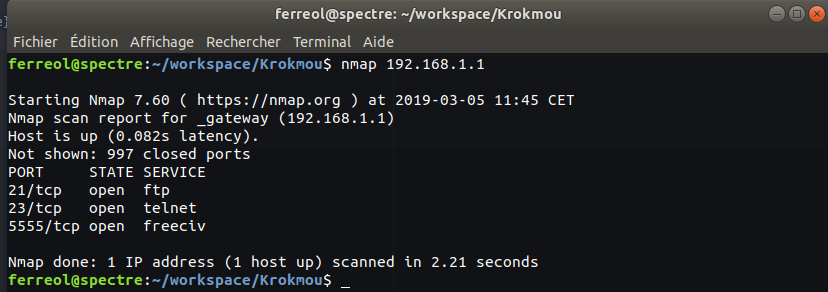
\includegraphics[scale=0.5]{images/scan_drone}
  \caption{Services disponibles sur le drone}
\end{figure}

La solution la plus simple serait de supprimer ces deux services et de les remplacer par un seul et même service, le service \textbf{ssh}. En effet, le service \textbf{ssh} combine l'aspect transfert de fichier de \textbf{ftp} et l'accès à distance de \textbf{telnet} et il offre en plus des garanties de sécurité avec notamment la présence d'un authentification à la connexion. Attention cependant, cette solution n'est viable que si le mot de passe par défault est changé à la première utilisation du drone.
